\documentclass[12pt,twoside=off,
bibtotoc,liststotoc,appendixprefix,paper=a4,headings=small]{scrbook} % 'twoside=on' für Druckversion oder 'twoside=off' für Onlineversion

%
% Packages
% -----------------------------------
\usepackage[
  paper=a4paper,
  left=12.5mm,
  right=25mm,
  top=25mm,
  bottom=50mm,
  bindingoffset=10mm]{geometry}		% Seitenränder und Bindungskorrektur einstellen
  
\usepackage{apacite} 			
\usepackage{svg}% Literatur-Referenzen: American Psycholog. Assoc.
\usepackage{natbib}
\usepackage{pdfpages}
\usepackage{graphicx}
\usepackage{float}
\setcitestyle{round,aysep={}} 		% Indizierg. in runden Klammern, zw. Autor u. Jahr
\usepackage[utf8]{inputenc}         % Umlaute im Text
\usepackage[english]{babel}

\usepackage[T1]{fontenc}
\usepackage{lmodern}				% Schriftfamilie
\usepackage{microtype}				% für die Mikrotypografie (besseres Schriftbild)
\setkomafont{disposition}{\bfseries}

\usepackage{graphicx} 				% Grafiken einfügen (pdf,png - aber jpg vermeiden)
\graphicspath{{./Bilder/}}          % Pfad zu den Bildern

\usepackage{url}					% URL's formatieren (z.B. in Literatur) 
\usepackage[colorlinks,linkcolor=black,citecolor=black,urlcolor=black]{hyperref} 				% für Hyperlinks in PDF-Dokumenten   
  
\usepackage{tabularx} 				% bessere Gestaltung von Tabellen
\usepackage{longtable} 		
\usepackage{multicol}				
\usepackage{multirow}
\usepackage{booktabs}
\usepackage{tabularx}
		
\usepackage[active]{srcltx}

\usepackage{listings}				% Algorithmen

\usepackage{mdwlist}				% Listen

\usepackage{setspace} 				% Zeileneinstellung
\newtheorem{mydef}{Merksatz}  		% Falls Beispiele, Merksätze m. fortl. Nr. gebr. werden
\newtheorem{bsp}{Beispiel}

\usepackage{todonotes}				% zum Erstellen von ToDos im Editor

\usepackage{lscape}					% zum Rotieren von Seiten

\usepackage{amsmath}				% zum Schreiben von mathematischen Formeln

\usepackage{calc}

\usepackage{footnote}				% Fußnoten
\usepackage{tablefootnote}			% Fußnoten in Tabellen

%\clubpenalty = 10000
%\widowpenalty = 10000 \displaywidowpenalty = 10000

\hyphenation{voll-st\"andigen}		% Worttrennungen global definieren

\setcounter{tocdepth}{1}			% Ebenen, die im Inhaltsverzeichnis angezeigt werden

% Document
% -----------------------------------
\begin{document}

\frontmatter 
    % Titelseite soll keine Kopf oder Fußzeile haben
\thispagestyle{empty}

% Alle Elemente sollen zentriert sein
\begin{center}

\vspace*{-5mm}

{\LARGE INTERNSHIP REPORT \\[1mm]}
% ANEVIS SOLUTIONS\\

\vspace*{2cm}


\includegraphics[width=0.35\textwidth]{Bilder/anevis_logo_big.png}

% \vspace*{1cm}

% % Art der Arbeit => (Bachelorarbeit ,Diplomarbeit, Masterarbeit, Seminararbeit)
% {\Large \textbf{Mandatory Internship}}\\ 

\vspace{1.5cm}

% Titel der Arbeit 
{\Large \textbf{Implementation of a Factsheet Reporting Project}}\\ 
\vspace*{1mm}
{\Large \textit{The creation of reports for a financial product}}\\ 
\vspace*{1mm}
{\Large \textit{for banks and fund managers}}\\

\vspace{1.2cm}

% Name des/der Autors/Autoren
{\LARGE Irmak Damla Özdemir}\\[15mm]
\vspace{1.6cm}
% Gutachter, Kontaktdaten und Abgabetermin
\hspace*{1.3cm}
\parbox{120mm}{
\begin{large}
\begin{tabbing}
Duration: \hspace{3.7cm} 10. Feb 2026 - 17. Jul 2026\\
Internship Coordinator: \hspace{.7cm} \=Prof. Dr.-Ing. Erik Schaffernicht\\
Project Manager:\> Sebastian Kempf\\[4mm] % alphabetische Reihenfolge (Nachname)
Student ID:\> 5123127\\
% Adresse:\> , 97076, Würzburg, Germany\\
E-mail:\> irmakozfecontact@gmail.com\\
Phone:\>0049 1575 462 59 32\\
Semester:\> Summer Semester 2026\\
Field of Study:\>B. Eng. Computer Science\\
University:\> Technical University of Applied Sciences\\ \>Würzburg-Schweinfurt\\[8mm]
Submission Date: \> 01. September 2026\\
\end{tabbing}
\end{large}
}

\end{center}
\clearpage{\pagestyle{empty}\cleardoublepage}
 			% Titelblatt
    \thispagestyle{empty}


\vspace*{1cm}

\begin{center}
    \textbf{Abstract}
\end{center}

\vspace*{1cm}

This report presents a compherensive analysis of my internship experience at Anevis Solutions, a leading reporting provider. The primary focus of the internship was to understand and implement IT-based automated reporting solutions for the financial sector. tbd\\

The internship provided an invaluable opportunity to apply theoretical knowledge acquired in academic students to real-world scenarios. I participated in several projects, notably the "Christian Hintz Vermögensverwaltung AI Leaders Factsheet Reporting", which aimed to provide individual and dynamic reporting for their fund investment class.\\

Additionally, the experience offered a better understanding of Linux systems, Bash scripts, database management and charting libraries like JFreeChart. I implemented various so called parsers to contribute automation of reportings. This Parser types were used to take the data from customer as any file type and save it consistently to the databases and then fetch the data from the database and create charts and analytics for reportings via Jaspersoft Studio.\\  

The intership underscored the importance of adaptability, teamwork and continuous learning. It also highlighted the critical role of clean and reusable implementation for the maintainability of distributed systems.(?) Furthermore, it reinforced my passion to develop sustainable, reusable and customized software for IT Technologies and has shaped my career aspirations in Backend Development.\\

This report details the project undertaken, skills developed and lessons learned throughout the internship, within a very organized work culture and with constant feedbacks from colleagues and supervisor.



 	% Abstract auf Deutsch 
    \newpage
    \clearpage{\pagestyle{empty}\cleardoublepage}
    \thispagestyle{empty}

\vspace*{1cm}

\begin{center}
    \textbf{Abstract}
\end{center}

\vspace*{1cm}

\noindent 
Dieser Bericht präsentiert eine umfassende Analyse meines Praktikums bei Anevis Solutions, einem Anbieter im Bereich Reporting-Lösungen. Der Schwerpunkt des Praktikums lag auf dem Verständnis und der Implementierung IT-basierter automatisierter Reporting-Lösungen für den Finanzsektor.\\\\
Das Praktikum bot eine wertvolle Gelegenheit, theoretisch erworbenes Wissen aus dem Studium in realen Anwendungen einzusetzen. Dabei arbeitete ich an mehreren Projekten mit, insbesondere am Projekt „Christian Hintz Vermögensverwaltung AI Leaders Factsheet Reporting“, das darauf abzielte, individuelle und dynamische Berichte für eine bestimmte Investmentfonds-Klasse bereitzustellen.\\\\
Darüber hinaus ermöglichte die Tätigkeit ein vertieftes Verständnis von Linux-Systemen, Bash-Skripten, Datenbankmanagement sowie Charting-Bibliotheken wie JFreeChart. Im Rahmen der Automatisierung von Reporting-Prozessen implementierte ich verschiedene Parser-Typen. Diese dienten dazu, Kundendaten in unterschiedlichen Dateiformaten zu verarbeiten, konsistent in Datenbanken zu speichern und anschließend für die Erstellung von Diagrammen und Analysen in Jaspersoft Studio wieder abzurufen.\\\\
Das Praktikum verdeutlichte die Bedeutung von Anpassungsfähigkeit, Teamarbeit und kontinuierlichem Lernen. Zudem wurde die Relevanz sauberer und wiederverwendbarer Implementierungen für die Wartbarkeit verteilter Systeme hervorgehoben. Diese Erfahrungen stärkten mein Interesse an der Entwicklung nachhaltiger, wiederverwendbarer und maßgeschneiderter Softwarelösungen im IT-Bereich und prägten meine beruflichen Ziele in der Backend-Entwicklung.\\\\
Dieser Bericht dokumentiert die durchgeführten Projekte, die erworbenen Fähigkeiten sowie die gewonnenen Erkenntnisse während des Praktikums in einem strukturierten Arbeitsumfeld mit kontinuierlichem Feedback durch Kollegen und Vorgesetzte.

    \newpage
     \clearpage{\pagestyle{empty}\cleardoublepage}
    \thispagestyle{empty}


\vspace*{1cm}

\begin{center}
    \textbf{Approval}
\end{center}

\noindent
\textbf{Approved By}
\vspace*{0.7cm} \\
\textbf{Company Supervisor}
\vspace*{1cm} \\ \\
\hspace*{-0.5cm}%
\dotfill\\
Name \hspace{5cm} Signature \hspace{3cm} Date\\\\\\
\textbf{Academic Supervisor}
\vspace*{1cm} \\ \\
\hspace*{-0.5cm}%
\dotfill\\
Name \hspace{5cm} Signature \hspace{3cm} Date\\\\
\hspace*{8.5cm}%

\noindent 

    \newpage

    \clearpage{\pagestyle{empty}\cleardoublepage}
    \thispagestyle{empty}


\vspace*{1cm}

\begin{center}
    \textbf{Confidentiality Statement}
\end{center}

\vspace*{1cm}

\noindent 
I hereby confirm that confidential information obtained has been handled appropriately and has not been disclosed without permission.


\vspace{2cm}

\noindent
Würzburg, den XX July 2026

\vspace{3cm}

\hspace*{7cm}%
\dotfill\\
\hspace*{8.5cm}%
\textit{Sebastian Kempf / responsible person}      % Sperrvermerk
    \newpage
    
    \clearpage{\pagestyle{empty}\cleardoublepage}
    \onehalfspacing                  	% Zeilenabstand ab hier 1.5 zeilig
    \tableofcontents 					% Inhaltsverzeichnis
    \clearpage{\pagestyle{empty}\cleardoublepage} 
    
    \listoffigures 					 	% Abbildungsverzeichnis
    \clearpage{\pagestyle{empty}\cleardoublepage}
    
    \listoftables						% Tabellenverzeichnis
    \clearpage{\pagestyle{empty}\cleardoublepage}

% -----------------------------------
\mainmatter 							% die einzelnen Kapitel
    \chapter{Introduction}

Computer science has become one of the most important fields in today’s world due to the rapid digital transformation and the strong technology sector in Germany. Software development and information technologies play an essential role across almost every industry. As a result, computer engineers are expected not only to have solid theoretical knowledge but also practical experience in real-world applications.

For me, applying the theoretical knowledge gained during my studies to real projects has always been of great importance. Germany’s practice-oriented education system and the opportunities offered by THWS were key factors in my decision to study here. Through my internship, I had the opportunity to further develop my technical skills as well as gain valuable insight into the professional working environment in Germany.

\section{Motivation}
During my search for a suitable internship, several factors played an important role in my decision-making process. Gaining technical experience, working within a team under a structured project environment, and improving my personal weaknesses were key criteria for selecting my internship placement. In particular, I aimed to deepen my knowledge of a programming language and further develop my technical skill set.

One aspect that particularly stood out to me at Anevis was the structured way of working, including regular meetings, clearly defined task distribution, and the opportunity to independently complete assigned responsibilities. Another important motivation for me was the chance to adapt to and work within an existing software system. This was especially relevant, as I recognized that integrating into an already established codebase is more challenging than developing a project from scratch.

Overall, this experience represented an important step for me in improving my ability to work in a team, adapt to existing systems, and develop a more disciplined and structured approach to software development.
    \clearpage{\pagestyle{empty}\cleardoublepage}		% löscht Kopfzeilen und Seitennummerierung von der letzten Seite eines Kapitels, sofern dort kein Text mehr steht
    \chapter{Company Overview}

\section{Description}
Anevis Solutions GmbH is a software company based in Würzburg, Germany, specializing in digital reporting solutions for the financial industry across Europe. The company is a leading reporting provider, offering software and services that support banks, asset managers, fund providers, and other financial institutions in automating and optimizing their reporting processes while reducing manual effort.
\section{Products}

\subsection{Marketing Suite}

\textbf{Factsheets:} Automated generation of standardised fund and portfolio factsheets based on up-to-date financial data.\\
\textbf{Institutional Reporting:} Creation of detailed reports for institutional investors including performance and portfolio information.\\
\textbf{Sales Presentations:} Generation of customised presentation materials for client communication and sales activities.\\
\textbf{ESG Reporting:} Production of sustainability-related investment reports based on ESG data.\\
\textbf{Website Widgets:} Interactive components displaying live fund data and performance metrics on websites or client portals.\\
\textbf{Live Hosting for Documents:} Digital distribution and hosting of dynamically updated reports and marketing materials.

\subsection{Regulatory Suite}

\textbf{UCITS KIID:} Automated generation of Key Investor Information Documents for UCITS funds.\\
\textbf{PRIIPs KID / MiFID II:} Standardised regulatory disclosure documents for EU compliance requirements.\\
\textbf{FIDLEG BIB:} Regulatory reporting solution aligned with Swiss financial regulation.\\
\textbf{SFDR Reporting:} Sustainability disclosure reporting in accordance with SFDR requirements.\\
\textbf{PAI and EET Reporting:} Reporting of Principal Adverse Impacts and ESG template data.\\
\textbf{AIFMD Annex IV Reporting:} Regulatory reporting for Alternative Investment Fund Managers.\\
\textbf{Solvency II TPT:} Reporting solution for insurance sector regulatory requirements.

\subsection{Data Management Suite}

\textbf{Datawarehouse:} Centralised storage and management of financial and market data.\\
\textbf{Data Integration:} Integration and harmonisation of multiple internal and external data sources.\\
\textbf{Data Validation:} Ensures consistency, accuracy, and quality of input data.

\subsection{Risk \& Compliance Suite}

\textbf{Risk Management Service:} Portfolio risk analysis and exposure monitoring.\\
\textbf{Transaction Cost Calculation:} Calculation of transaction costs for performance and regulatory reporting.\\
\textbf{Market Conformity Check / Best Execution:} Analysis of trade execution quality and market conformity.\\
\textbf{Valuation \& Pricing Service:} Automated valuation and pricing of financial instruments.

\section{Departments}
\subsection{Sales \& Marketing}
\subsection{Human Resources}
\subsection{Operations}
\subsubsection{Project Management (PM)}
\subsubsection{Operations-Development (OPSDEV)}
Mission is to take care of the technical implementation of projects and technical support for OPS.
\subsubsection{Development (DEV)}
\subsubsection{Quality Assurance (QA)}


\section{TechStack and Tools}

\begin{figure}[H]
\centering

\begin{tabular}{ccc}



\includegraphics[width=2.5cm]{Bilder/java.png} &

\includegraphics[width=2.5cm]{Bilder/mongodb.png} &

\includegraphics[width=2.3cm]{Bilder/postgresql.png} \\


\includegraphics[width=2cm]{Bilder/js.png} &

\includegraphics[width=2.5cm]{Bilder/bash.png} &

\includegraphics[width=2.7cm]{Bilder/jaspersoft.png}
 \\



\includegraphics[width=2.5cm]{Bilder/git.png} &

\includegraphics[width=2.5cm]{Bilder/atlassian.png} &

\includegraphics[width=2.5cm]{Bilder/ubuntu.png}
\\

\end{tabular}

\caption{Technologies Used in the Company}
\end{figure}

\section{Team Events}

\subsection{Student Event SS 26}
An evening with all students (working students and interns), including short presentations, mini-games, and a shared dinner.

\subsection{OPS Team Event}
An evening in Steinbachtal, Würzburg. We had an archery session and competed in teams. Afterwards, we had dinner and desserts together at Schützenhof.

% 
\includegraphics[width=2.5cm]{Bilder/jira.png} &
% 
\includegraphics[width=2.5cm]{Bilder/confluence.png} &
    \chapter{Tasks in the Company}
The internship includes a broad range of side tasks in addition to the main internship project, providing real-world working experience and insight into office culture.

\section{Meetings}

\subsection{OPSDEV Daily Stand-up}
Every morning at 09:05, a short meeting is held via Google Meet where team members share updates on their current work and discuss ongoing tasks.
\subsection{OPSDEV Check-in Meetings}
Biweekly development team check-in meetings focusing on progress, challenges, concerns, achievements, and overall well-being, with all discussions recorded in the OPSDEV meeting protocols.
\subsection{OPS Review / Consultation Meetings}
Regular OPS team sessions where team members can ask questions, discuss issues, and receive support regarding Anevis products.
\subsection{Quarterly Reviews}
Quarterly review meetings are held where each team presents its current progress, key achievements, and ongoing activities in a structured, sequential manner. The meetings serve to provide an overview of the overall project status across all teams.
\subsection{Internship Feedback Sessions}
Feedback sessions were conducted at regular intervals throughout the internship to exchange mutual feedback, review overall progress, and discuss expectations and satisfaction levels from both sides.

\section{Onboarding}

\subsection{Onboarding Presentation from HR}
The onboarding presentation provided an introduction to Anevis and covered its history, organizational structure, office environment, and company culture. It also included information about meetings, team events, internal communication practices, as well as an overview of the company's products, tools, and working guidelines.

\subsection{OPSDEV Training Exercises}

\begin{itemize}
\item \textit{Exercise Streams:} A set of exercises designed to strengthen proficiency with Java Streams, reflecting their extensive use within the internal system and covering common stream operations and data processing patterns.
\item \textit{Exercise Databases:} Practical exercises focused on gaining experience with MongoDB and PostgreSQL, which are the primary databases used within the internal system, including querying, data modelling, and basic database operations.
\item \textit{Exercise Spring JPA:} An exercise focused on Spring, Hibernate, JPA, SQL, and Java. The task involved generating pie and ring charts with JFreeChart, exporting them to PDF, applying clean OO design principles, and supporting the solution with unit tests, streams, and lambdas.
\item \textit{Exercise Factsheet Project:} A practical factsheet generation exercise simulating a syntetic client project. The task involved working with the internal repositories like document engine, setup scripts; and Git workflows, real databases, JFreeChart reporting components to produce a complete factsheet in a dedicated development branch.

\end{itemize}

\section{OPSDEV - Daily Development Tasks}

\subsection*{OPSDEVBOX Tasks}

OPSDEVBOX taskleri automatisierungta onemli rol oynayan sirketin kendi internal sistemi icin implemente edilen tasklerdir.
Ornegin musteriden gelen datalarin veri bankasina nasil kaydedilecegi, database structurelari update edilmesi yani repositorylerdeki genel duzenlemeler bu task basligi altinda yapilir 


\begin{table}[H]
\centering
\begin{tabular}{p{4cm} p{10cm}}
\toprule
\textbf{Task} & \textbf{Description} \\
\midrule

\texttt{OPSDEVBOX-651} & Add region ultimo mapping to the project setup \\
\texttt{OPSDEVBOX-678} & Make category mandatory in project setup parser \\
\texttt{OPSDEVBOX-679} & Fix marketing classifications with empty identifiers \\
\texttt{OPSDEVBOX-662} & Move series from definitions data to series mappings \\
\texttt{**LLBSWISS-255} & Implement parser to insert valor \\

\bottomrule
\end{tabular}
\caption{OPSDEVBOX Tasks Overview}
\label{tab:opsdevbox-tasks}
\end{table}




\subsection*{BANTLEON Fast Charting Project}

Fast Charting Projesi, Bantleon sirketine ait esg report projesi icin ops team tarafindan hizli ve efektif bir sekilde chart uretimini saglayan databasele baglantisi olmayan pratik yardimci bir tool olarak gelistirilmistir.
Özetle bu class ile chartlar customization ile dilenildigi sekilde visualize edilebilir.

Iste bazi chart ornekleri:

\begin{figure}
    
\end{figure}

\begin{table}[H]
\centering
\begin{tabular}{p{4cm} p{10cm}}
\toprule
\textbf{Task} & \textbf{Description} \\
\midrule
\texttt{BANTLEON-249} & fast-charting-for-bantleon-esg-report \\
\bottomrule
\end{tabular}
\end{table}


\subsection*{Monitoring-Reporter}

Sirkette internal sistem kontrolunu saglamak ve bunlari dilenilen araliklarla mailde raporlastirmak icin bir servis bulunmaktadir ve burada ihtiyaca gore duzenli raporlar uretilebilmektedir.
Burada benim gorevim, sirketin databaseinde bulunan project componenti olmayan projeleri saptamak ve onlarin bilgisini bir tablo halinde mail olarak yonlendirmekti.
Burada internal sistemde zaten hali hazirda var olan bir Class i extend ederek customize edip bir reporter implemente ettim

\begin{table}[H]
\centering
\begin{tabular}{p{4cm} p{10cm}}
\toprule
\textbf{Task} & \textbf{Description} \\
\midrule

\texttt{OPSDEVBOX-680} & monitor-dead-projects \\
\bottomrule
\end{tabular}

\label{tab:opsdevbox-tasks}
\end{table}

\subsection*{Customer-specific Tasks}

Customer specific taskler, pm in musterilerden aldiklari geri bildirim ve taleplere yonelik olusturulan cesitli tasklerdir. 
Bunlara ornek olarak bir musterinin adinin, product adinin degistirilmesi, chartlarin legendinin 2 sutunlu yapilmasi, proje componenti silinmesi, static data update edilmesi, basketlerin ve pricelarin update edilmesi, vb.   
Özetle internship projecte oranla kapsami cok daha kucuk olan yan taskler. 


\section{Additional}
\subsection*{Confluence Article about JFreeCharts}
\subsection*{ISO 27001 Certification Training}
\subsection*{General Data Protection Awareness Training}
\subsection*{Anecon Support}
The perfect opportunity for networking in the financial service industry
Yilda bir kere duzenlenen, cesitli banka ve fon sirketlerinden konusmacilarinin oldugu, \dots
18 Haziran 2026 dan gerceklesen bu konferansta city helper olarak gorev aldim 
\subsection*{Cleaning Service (maybe)}

\section{Given Materials}
The following books were used as reference material during the internship:


\begin{itemize}
    \item Robert C. Martin: \textit{Clean Code: A Handbook of Agile Software Craftsmanship}
    \item Raoul-Gabriel Urma, Mario Fusco, Alan Mycroft: \textit{Java 8 in Action}
\end{itemize}

    \clearpage{\pagestyle{empty}\cleardoublepage}
    \chapter{Internship Project}


\section{Customer Overview}
Christian Hintz Vermögensverwaltung GmbH is an independent German asset management company based in Stuttgart. The firm specializes in providing discretionary wealth management services for private investors and businesses, focusing on individually tailored investment strategies and portfolio management. Operating as a regulated financial institution under the supervision of the German Federal Financial Supervisory Authority (BaFin), the company offers services such as strategic portfolio management, financial planning, and investment advisory with a strong emphasis on long-term, goal-oriented wealth building.
\section{Preparation}
\section{Requirements}
\section{Implementation}
\subsection{Setup Scripts}
\subsection{Services}
\subsection{Document Engine}

\subsubsection{Input Parser}

\subsubsection{Charting}

\subsubsection{Factsheet Parser}

\section{Testing}
    \clearpage{\pagestyle{empty}\cleardoublepage}
\chapter{Conclusion}

Lorem ipsum dolor sit amet, consectetuer adipiscing elit. 

\section{Learning Outcomes}


Nullam sagittis ... 
    This is a test citation \cite{Fiig2004}.
    \clearpage{\pagestyle{empty}\cleardoublepage}
   
    \clearpage{\pagestyle{empty}\cleardoublepage}
     \chapter{AI List}

The following table lists the artificial intelligence tools used in this report:

\begin{table}[h!]
\centering
\begin{tabular}{|l|l|l|}
\hline
\textbf{AI Tool} & \textbf{Purpose} \\
\hline
ChatGPT & Text translation and correction \\
\hline
Claude & LaTeX correction \\
\hline
\end{tabular}
\caption{AI tools used in the project}
\end{table}
     \clearpage  
 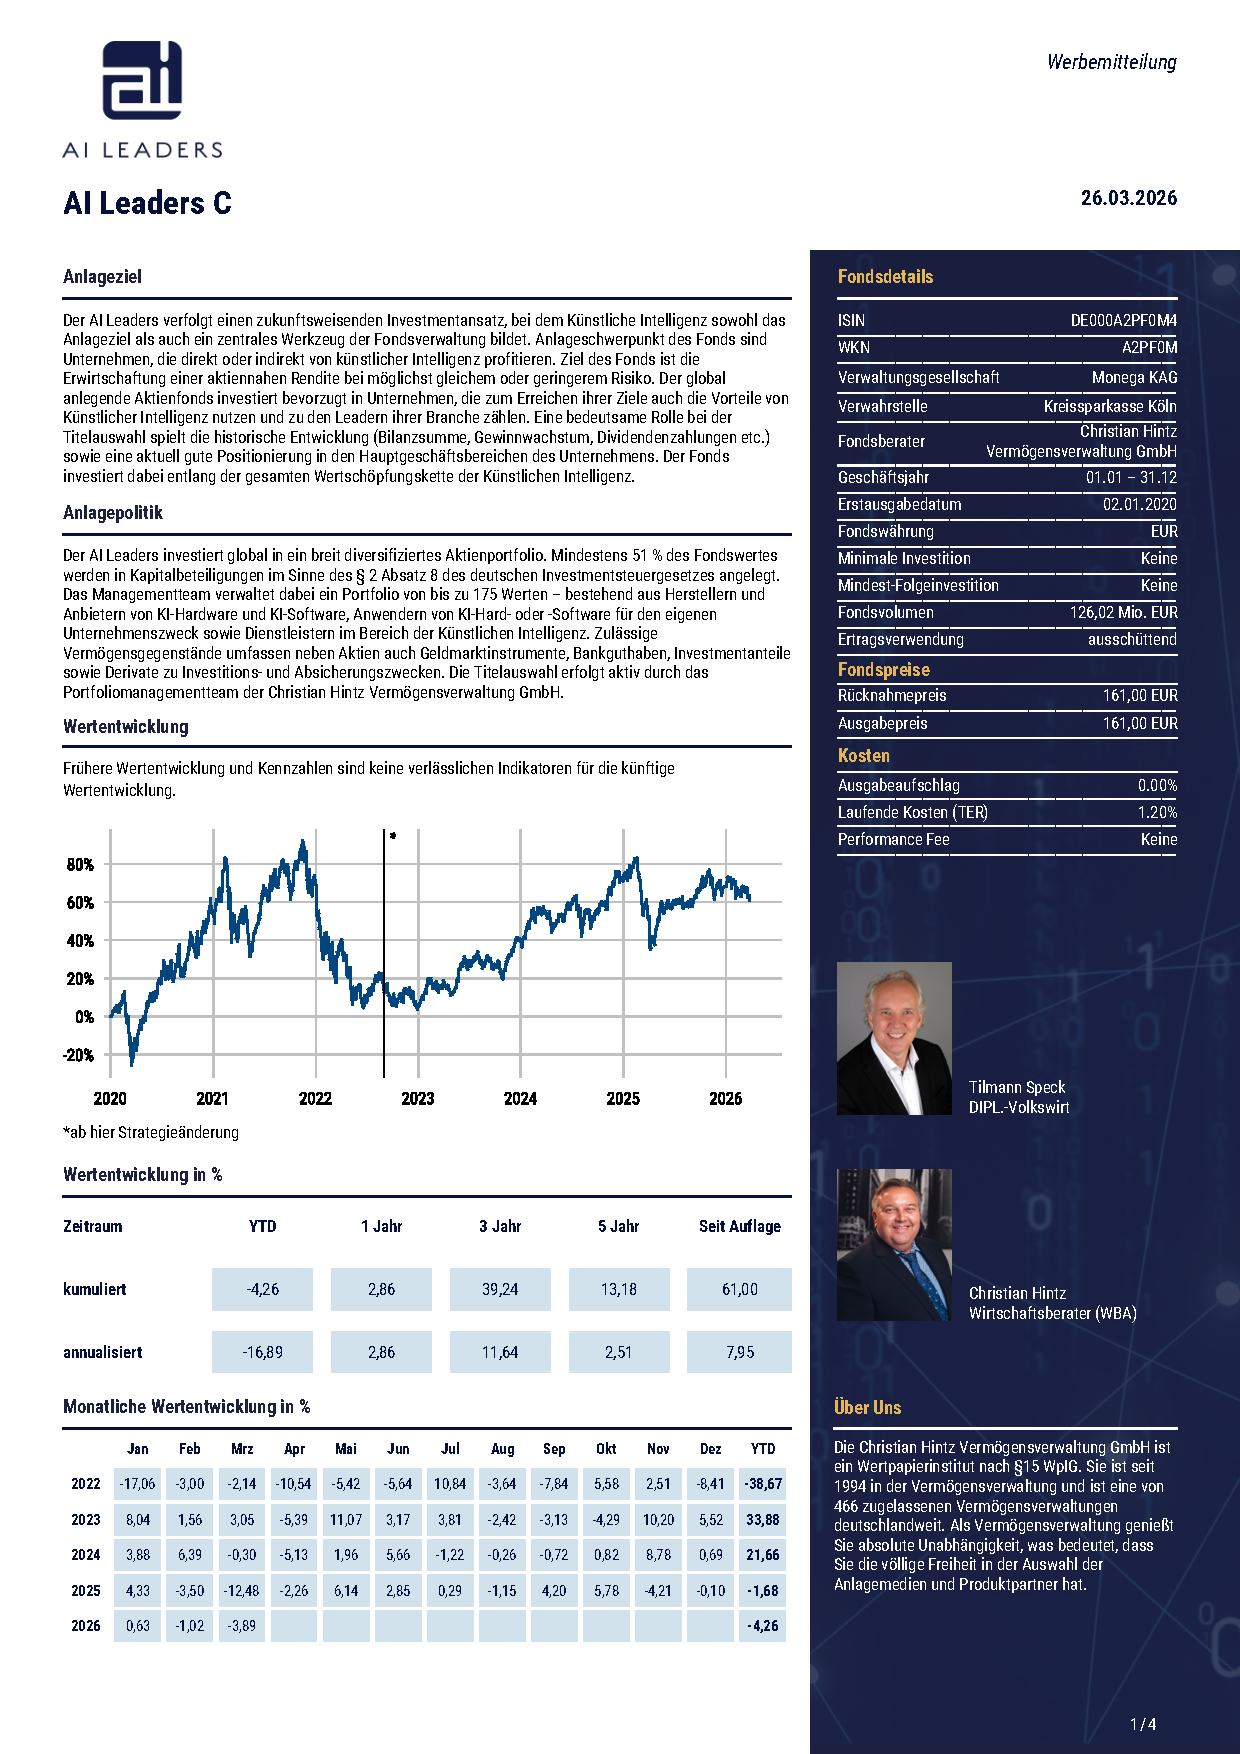
\includepdf[pages=-]{aiLeaders.pdf}
 \addcontentsline{toc}{chapter}{AI Leaders C Factsheet}


% -----------------------------------
\backmatter 
\bibliographystyle{apacite}				% bei natbib in deutsch
\bibliography{./Literatur/quellen}		% Literaturquellen einbinden 
\newpage
\thispagestyle{empty}
\noindent

I hereby confirm that:
\begin{itemize}
    \item I have independently prepared the submitted work, and
    \item I have not used any additional sources other than those explicitly permitted and indicated in advance
\end{itemize}

\vspace{2cm}

\noindent
Würzburg, \today

\vspace{3cm}

\hspace*{7cm}%
\dotfill\\
\hspace*{8.5cm}%
\textit{Irmak Damla Özdemir} 			% Eidesstattliche Erklärung (nicht bei Seminararb.)

\end{document}